\documentclass[article,colorback,accentcolor=tud2c]{tudreport}
\usepackage{ngerman}

\usepackage[stable]{footmisc}
\usepackage[ngerman]{hyperref}
\usepackage[utf8]{inputenc}

\usepackage{longtable}
\usepackage{multirow}
\usepackage{booktabs}

\setlength{\parindent}{0pt}

\hypersetup{%
  pdftitle={Zeiterfassungsportal für HiWis},
  pdfauthor={Jan Dillmann, Fabian Letzkus, Stephan Moczygemba},
  pdfsubject={Setup-Information},
  pdfview=FitH,
  pdfstartview=FitV
}

\setcounter{seclinedepth}{1}

%%% Zum Tester der Marginalien %%%
  \newif\ifTUDmargin\TUDmarginfalse
  %%% Wird der Folgende Zeile einkommentiert,
  %%% werden Marginalien gesetzt.
  % \TUDmargintrue
  \ifTUDmargin\makeatletter
    \TUD@setmarginpar{2}
  \makeatother\fi
%%% ENDE: Zum Tester der Marginalien %%%

\newlength{\longtablewidth}
\setlength{\longtablewidth}{0.7\linewidth}
\addtolength{\longtablewidth}{-\marginparsep}
\addtolength{\longtablewidth}{-\marginparwidth}


% \settitlepicture{tudreport-pic}
% \printpicturesize

\title{Zeiterfassung für HiWis}
\subtitle{Setup-Information}
\subsubtitle{Jan Dillmann\\Fabian Letzkus\\Stephan Moczygemba}
%\setinstitutionlogo[width]{TUD_sublogo}
\uppertitleback{(\textaccent{\textbackslash uppertitleback})}
\lowertitleback{(\textaccent{\textbackslash lowertitleback})\hfill\today}

\begin{document}
\maketitle

\tableofcontents

\newpage

\section{Das Projekt} % (fold)
\label{sec:das_projekt}

Das Projekt ``Zeiterfassungsportal für HiWis'' wurde im Rahmen des Internet-Praktikums des Fachbereichs Telekooperation der TU Darmstadt im Sommersemester 2011 von Jan Dillmann, Fabian Letzkus und Stephan Moczygemba entwickelt.

Zweck des Portals ist es, den Mitarbeitern aller Fachbereiche eine Übersicht ihrer studentischen Mitarbeiter (``HiWis'') zu geben sowie deren Aufgaben zu verwalten.

Studentische Mitarbeiter, welche ebenfalls Zugriff auf dieses Portal erhalten, können ihren Zeitaufwand pro Aufgabe erfassen und erhalten ebenso wie die Mitarbeiter der Fachbereiche eine Übersicht ihrer gearbeiteten bzw. noch zu leistenden Stunden.

% section das_projekt (end)

\section{Verwendete Technologien} % (fold)
\label{sec:verwendete_technologien}

Im Projekt werden verschiedene Technologien eingesetzt. Diese sind im einzelnen:

\begin{itemize}
    \item Hibernate\footnote{\url{http://www.hibernate.org/}} als Abstraktionsschicht zur Datenbank
    \item extJS\footnote{\url{http://www.sencha.com/products/extjs/}} als Client-Framework für die GUI
    \item JOpenID\footnote{\url{http://code.google.com/p/jopenid/}} zur Benutzerauthentifizierung
    \item Resteasy\footnote{\url{http://www.jboss.org/resteasy}} zur Bereitstellung eines REST-Servers für extJS
\end{itemize}

% section verwendete_technologien (end)

\section{Projektstruktur} % (fold)
\label{sec:projektstruktur}

Der gesamte Quellcode des Projekts sowie die Dokumentation sind als öffentliches Repository auf dem Dienst \emph{GitHub}\footnote{\url{https://github.com}} unter der URL \url{https://github.com/SteMo/Zeiterfassung_HiWis_TUD} frei verfügbar.

Neben dem Kommandozeilen-Befehl \texttt{git} stehen Clients für verschiedene Betriebssysteme zur Verfügung, beispielsweise

\begin{itemize}
    \item Tower für OS X (\url{http://www.git-tower.com})
    \item SmartGit für Windows (\url{http://www.syntevo.com/smartgit/index.html})
\end{itemize}

Um den Quellcode des Projekts zu erhalten kann das gesamte Repository geklont werden (zu finden unter \url{git@github.com:SteMo/Zeiterfassung_HiWis_TUD.git}).

% section projektstruktur (end)

\section{Projekt-Setup in Eclipse} % (fold)
\label{sec:projekt_setup_in_eclipse}

Das Projekt kann mit Hilfe des Build-Management-Tools \emph{Maven}\footnote{\url{http://maven.apache.org/}} erstellt werden. Für die Integration in \emph{Eclipse IDE}\footnote{\url{http://www.eclipse.org/}} werden die folgenden Plugins benötigt:

\begin{itemize}
    \item m2e (\url{http://download.eclipse.org/technology/m2e/milestones/1.0})
    \item m2e-wtp (\url{http://download.jboss.org/jbosstools/updates/m2eclipse-wtp})
\end{itemize}

Nach dem Clonen des Repositories (zu finden unter der URL ) kann das Projekt in Eclipse importiert werden.

Dazu ist der Befehl \texttt{Import} $\rightarrow$ \texttt{Maven} $\rightarrow$ \texttt{Existing Maven Projects} auszuführen. Als Root-Directory muss das Verzeichnis \texttt{de.tud.cs.tk.zeiterfassung} gewählt und unter \texttt{Advanced} $\rightarrow$ \texttt{Naming template} das Template \texttt{[groupId].[artifactId]} verwendet werden.

Wenn noch nicht vorhanden muss noch ein Apache Tomcat v6.0 Server installiert werden. Dazu kann im \emph{Servers}-View von Eclipse über \texttt{New} $\rightarrow$ \texttt{Server} ein solcher hinzugefügt werden.

Das Portal kann dann über \texttt{Run As} $\rightarrow$ \texttt{Run on Server} gestartet werden.

% section projekt_setup_in_eclipse (end)

\section{Datenbank-Setup} % (fold)
\label{sec:datenbank_setup}

Vom Portal verwaltete Daten werden in einer PostgreSQL-Datenbank gespeichert. Das voreingestellte Setup erwartet eine Datenbank namens \texttt{Zeiterfassung} mit dem Eigentümer \texttt{zeiterfassung} und dem Passwort \texttt{hiwi} auf dem PostgreSQL-Server \texttt{localhost:5432}.

Diese Daten können und sollten in der Datei \texttt{/src/main/resources/hibernate.cfg.xml} angepasst werden.

Beispieldaten können über \url{http://localhost:8080/zeiterfassung/install} automatisch in die Datenbank eingefügt werden. Diese Daten gliedern sich auf in reine Beispieldaten und Daten die fix für die Benutzung gesetzt bleiben müssen.

Die nötigen Daten umfassen die möglichen Rollen sowie die einen initialen Administrator. Alles Weitere kann über die Oberfläche angelegt werden (ein Administator muss für den initialen Login vorhanden sein und kann dann zusätzliche Personen anlegen).

Die Beispieldaten umfassen Aufgaben, Verträge, Fachgebiete und Personen. Hierbei werden drei Personen -- für jede Rolle eine -- angelegt. Die Daten sind momentan auf unsere OpenIDs ausgelegt, d.h. nur wir werden authentifiziert (und authorisiert). 

Für den initialen Administrator muss als dessen ``principal'' (Identifier zur Authentifizierung) die eigene OpenID eingetragen werden. Um sich hier selbst hinzuzufügen, müssen nur wenige Felder im Code entsprechend gesetzt werden:

Im Projekt unter ``Java Resources'' - \texttt{src/main/java/de/tud/cs/tk/zeiterfassung/Installation.java} können die (Beispiel-)Personen geändert werden. Insbesondere das Attribut ``principal'' muss auf die eigene OpenID gesetzt werden, um sich authentifizieren zu können.

Die eigene OpenID kann momentan wie folgt ermittelt werden:

\begin{enumerate}
    \item Öffnen der URL~\url{http://localhost:8080/zeiterfassung/JOpenIdTest}
    \item Authentifizieren gegenüber Google
    \item Nach erfolgreicher Authentifizierung die URL mit dem Schema \texttt{https://www.google.com/accounts/o8/id?id=...} kopieren und unter <person>.principal einfügen.
\end{enumerate}

Bevor man die Zeitverwaltungssoftware nun nutzen kann muss man sich bei Google einloggen, um die Authentifizierung über OpenID zu ermöglichen. Die Startseite lautet in der aktuellen Version je nach Rollenzugehörigkeit wie folgt:
\begin{itemize}
\item http://localhost:8080/zeiterfassung/?role=admin
\item http://localhost:8080/zeiterfassung/?role=mitarbeiter
\item http://localhost:8080/zeiterfassung/?role=hiwi
\end{itemize}

Möchte eine Person ihre Rolle wechseln, so muss momentan das Installationsskripts angepasst werden. Nach einer Änderung des Installationsskripts muss der tomcat-Server neu gestartet und anschließend \url{http://localhost:8080/zeiterfassung/install} erneut aufgerufen werden um eben die Datenbank entsprechend neu zu füllen.

% section datenbank_setup (end)

\newpage

\section{Screenshots} % (fold)
\label{sec:screenshots}

Das Dashboard eines als Mitarbeiter eingeloggten Benutzers bietet in erster Linie eine Übersicht der ihm zugeteilten studentischen Mitarbeiter sowie deren Aufgaben.

\begin{figure}[h]
    \begin{center}
        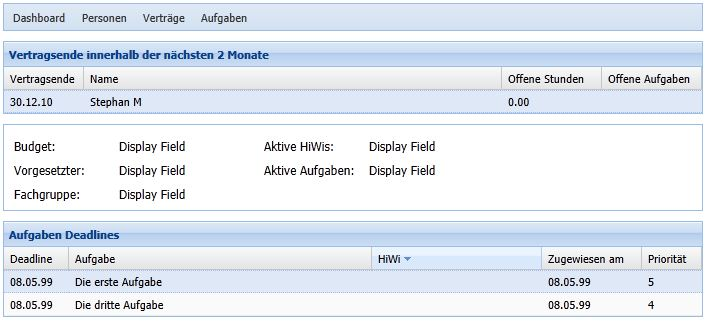
\includegraphics[scale=0.8]{img/mitarbeiter-dashboard}
    \end{center}
\end{figure}

\newpage

Neue Aufgaben können einzelnen HiWis mit Deadline und Priorität zugeteilt werden.

\begin{figure}[h]
    \begin{center}
        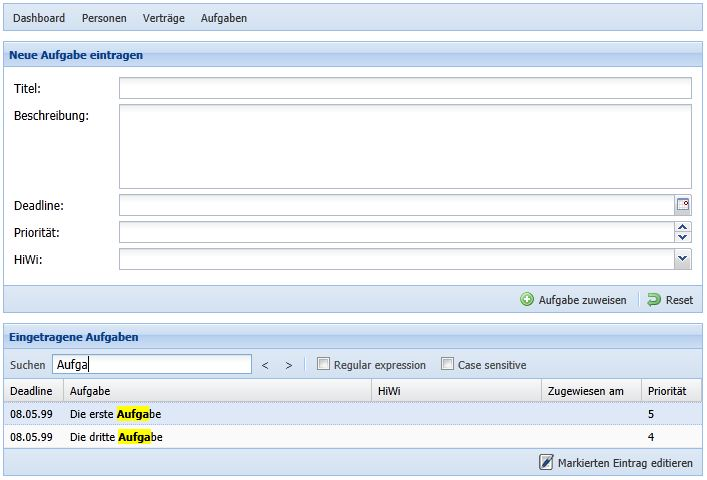
\includegraphics[scale=0.7]{img/mitarbeiter-aufgaben}
    \end{center}
\end{figure}

Studentische Mitarbeiter sehen eine Übersicht ihrer Aufgaben und können gearbeitete Stunden erfassen.

\begin{figure}[h]
    \begin{center}
        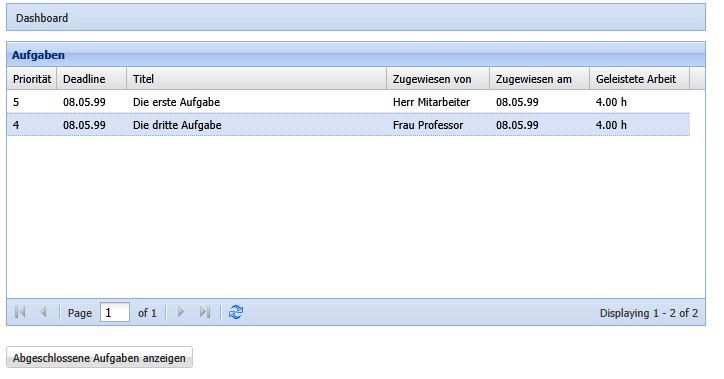
\includegraphics[scale=0.7]{img/hiwi-dashboard}
    \end{center}
\end{figure}

% section screenshots (end)

\newpage

\section{Datenbankschema} % (fold)
\label{sec:datenbankschema}

\begin{figure}[h]
    \begin{center}
        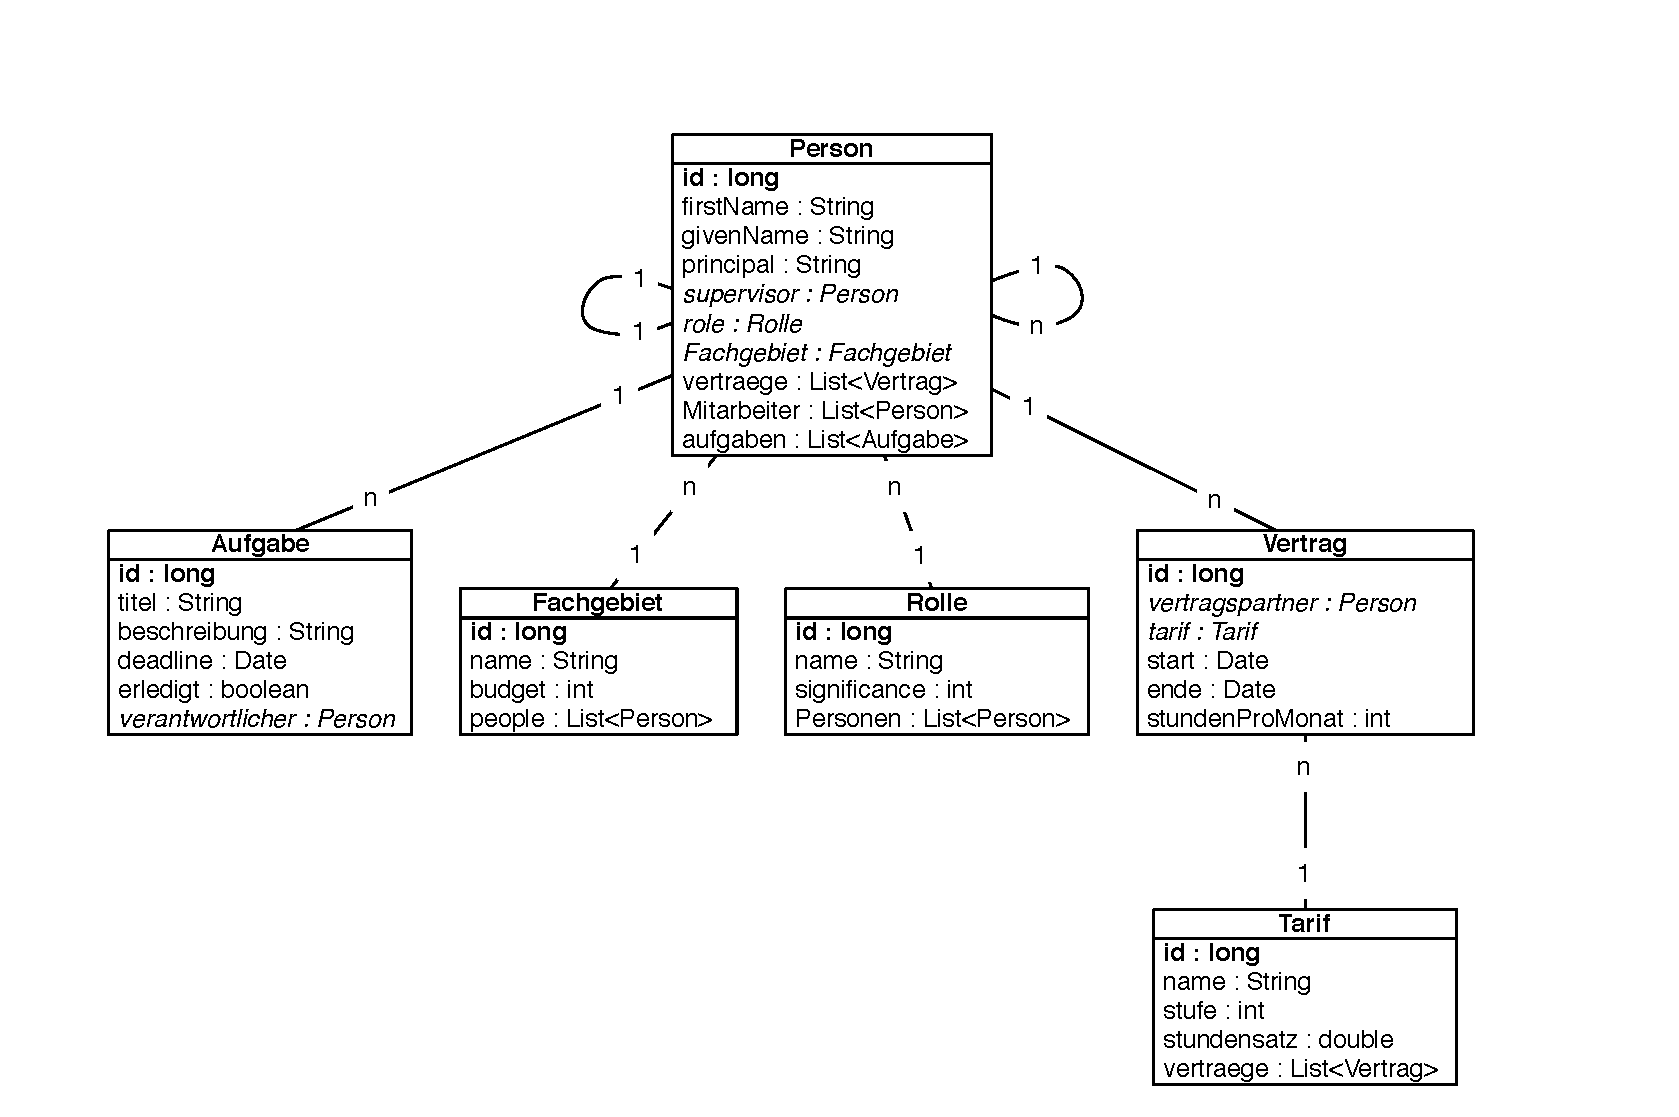
\includegraphics[scale=0.6]{img/db}
    \end{center}
\end{figure}

% section datenbankschema (end)

\end{document}
